\documentclass[utf8, diplomski, lmodern]{fer}

% font
\renewcommand{\familydefault}{\sfdefault}  % sans-serif main

%\usepackage{arev}
%\usepackage[cm]{sfmath}  % bolje nego mathastext
%\SetSymbolFont{largesymbols}{normal}{OMX}{iwona}{m}{n}

%\usepackage[italic]{mathastext}  % sfmath je bolje (manji indeksi)


%\usepackage{inconsolata}					% sans-serif monospace
\usepackage[scaled]{beramono}				% sans-serif monospace


%\usepackage[math]{iwona}
%\usepackage[math]{kurier}

\usepackage[T1]{fontenc}  % accented characters, copy from pdf, ...

\raggedright						% bez desnog poravnavanja

\usepackage{caption}
\captionsetup{%
	justification=raggedright,
}
\setlength{\parindent}{1em}	 % uvlačenje ulomaka
\usepackage{indentfirst}	 % uvlačenje prvog ulomka
\setlength{\parskip}{0.5em}	 % razmak između ulomaka

\usepackage{listings}  % listings
\renewcommand{\lstlistingname}{Ispis}

\usepackage[multiple]{footmisc}	 % višestruke fusnote

\usepackage[hidelinks]{hyperref}
\renewcommand*{\UrlFont}{\footnotesize}

% colors

\usepackage{xcolor}
\usepackage{color}

\hypersetup{
	colorlinks,
	linkcolor={blue!50!green!50!black},  % xcolor package
	citecolor={green!40!black},
	urlcolor={blue!75!green!30!black}
}
\definecolor{bluekeywords}{rgb}{0.13,0.13,1}  % color package
\definecolor{greencomments}{rgb}{0,0.5,0}
\definecolor{redstrings}{rgb}{0.9,0,0}

\let\emph\relax
\DeclareTextFontCommand{\emph}{\bfseries}

\newtheorem{theorem}{Teorem}[section]
\newtheorem{definition}{Definicija}[section]

\usepackage{enumitem}  % \begin{enumerate}[topsep=0pt,itemsep=0pt,partopsep=0pt]

% redefinition of left and right to make spacing consistent
\let\originalleft\left
\let\originalright\right
\def\left#1{\mathopen{}\originalleft#1}
\def\right#1{\originalright#1\mathclose{}}

\usepackage{amsmath}
\usepackage{mathtools}  % \coloneqq
%\usepackage{bm}
%\usepackage[utopia]{mathdesign}
\usepackage[OMLmathsfit]{isomath}  % \DeclareMathAlphabet ...
%\usepackage[bbgreekl]{mathbbol}

\usepackage{mathtools}  % smashoperator
\usepackage{commath}  % calculus, perentheses
\usepackage{stmaryrd}  % \llbracket for \rrbracket, ...

%\usepackage[croatian]{babel}		% teorem
%\newtheorem{definition}{Definicija}[section]
%\newtheorem{theorem}{Teorem}[section]
%\newtheorem{corollary}{Korolar}[theorem]

\DeclareMathAlphabet{\mathbbmsl}{U}{bbm}{m}{sl}
\DeclareMathAlphabet{\mathbbmb}{U}{bbm}{b}{it}
\DeclareMathAlphabet{\mathbbmssit}{U}{bbmss}{m}{it}


% common set?, distribution
\newcommand{\commset}[1]{\mathbbmb{#1}}
\newcommand{\distrib}[1]{\mathcal{#1}}

% sans-serif blackboard-bold
\newcommand{\mathsfbbit}[1]{\mathbbmssit{#1}}

% variable
\let\vec\relax
\let\set\relax
\newcommand{\vec}[1]{\mathbfit{#1}}
\newcommand{\mat}[1]{\vec{#1}}
\newcommand{\ten}[1]{\vec{#1}}
\newcommand{\set}[1]{\mathbbmsl{#1}}

% constant
\newcommand{\const}[1]{\mathrm{#1}}
\newcommand{\cvec}[1]{\mathbf{#1}}
\newcommand{\cmat}[1]{\cvec{#1}}
\newcommand{\cten}[1]{\cvec{#1}}
\newcommand{\cset}[1]{\mathbb{#1}}

% random variable
\newcommand{\rvar}[1]{{\color{blue!70!black}\mathsfit{#1}}}
\newcommand{\rvec}[1]{{\color{blue!70!black}\mathsfbfit{#1}}}
\newcommand{\rmat}[1]{\rvec{#1}}
\newcommand{\rten}[1]{\rvec{#1}}
\newcommand{\rset}[1]{{\color{blue!70!black}\mathsfbbit{#1}}}

% linear algebra
\newcommand{\transpose}{\mathsf T}

% calculus - commath: od, pd, md, dif
% parentheses - commath: del, cbr, sbr, envert, enVert

% named functions
\DeclareMathOperator{\softplus}{softplus}
\DeclareMathOperator{\softmax}{softmax}
\DeclareMathOperator{\logistic}{\sigma}
\DeclareMathOperator{\sgn}{sgn}
\DeclareMathOperator{\diag}{diag}

% operators
\DeclareMathOperator*{\argmin}{arg\,min} % thin space
\DeclareMathOperator*{\argmax}{arg\,max}
\DeclareMathOperator*{\E}{{\rm I\kern-.282em E}}
\DeclareMathOperator*{\D}{{\rm I\kern-.282em D}}
\DeclareMathOperator*{\Cov}{Cov}
\let\H\relax
\DeclareMathOperator*{\H}{{\rm H\kern-.8em H}}
\DeclareMathOperator*{\Dklsym}{D_{\mathrm{KL}}}

% bracket operators
\newcommand{\enangle}[1]{\mathinner{\left\langle{#1}\right\rangle}}
\newcommand{\enbbracket}[1]{\mathinner{\left\llbracket{#1}\right\rrbracket}}
\newcommand{\braket}[2]{\enangle{{#1}|{#2}}}

% parentheses from commath redefined to improve spacing because (left and right were redefined)
\renewcommand{\del}[1]{\left(#1\right)}
\renewcommand{\sbr}[1]{\left[#1\right]}
\renewcommand{\cbr}[1]{\left\{#1\right\}}
\renewcommand{\intoo}[1]{\mathinner{\del{#1}}}
\renewcommand{\intcc}[1]{\mathinner{\sbr{#1}}}
\renewcommand{\intco}[1]{\mathinner{\left[#1\right)}}
\renewcommand{\intoc}[1]{\mathinner{\left(#1\right]}}

% special
\newcommand{\funcdef}[3]{#1 \colon #2 \to #3}
\newcommand{\Dkl}[2]{\Dklsym\del{#1\;\middle\|\;#2}}
\newcommand{\C}{\cset{C}}
\newcommand{\R}{\cset{R}}
\newcommand{\Z}{\cset{Z}}
\newcommand{\N}{\cset{N}}
\newcommand{\dirac}{\delta}
\newcommand{\ind}[2]{#1_{\sbr{#2}}}

% operators
\newcommand{\bidot}{\mkern1.5mu{..}\mkern1.5mu}
\newcommand\sheq{\mkern1.5mu{=}\mkern1.5mu}
%\renewcommand{\dots}{...}
\usepackage{booktabs}  % from the tamplate; table quality enhancement

\usepackage{multirow}
\usepackage{tabularx}

\newcolumntype{P}[1]{>{\raggedright\let\newline\\\arraybackslash\hspace{0pt}}p{#1}}

\renewcommand{\arraystretch}{1.4}
%\usepackage{floatrow} 				% centriranje svih slika
\usepackage{float}					% figure [H]
\usepackage{graphicx} 				% includegraphics
\usepackage{caption}			% subfigure
\usepackage{subcaption}			% subfigure
\usepackage[export]{adjustbox} 	% http://ctan.org/pkg/adjustbox

\usepackage[section]{placeins}  % [section] for \FloatBarrier before every section 

\graphicspath{ {./figures/} }		% mapa sa slikama
%\let\oldincludegraphics\includegraphics
%\renewcommand{\includegraphics}[2][]{\oldincludegraphics[#1,max width=0.9\linewidth]{#2}}

%\usepackage{flafter} % floats after the first reference

\usepackage{tikz} 					% dijagrami
\usepackage{pgfplots}
\usetikzlibrary{fit,automata,arrows,positioning,calc,petri,topaths,arrows.meta}

%\usetikzlibrary{external}
%\tikzexternalize[prefix=figures/tikz/, shell escape=-enable-write18]
%TexStudio Configuration\commands\pdflatex:
%"pdflatex.exe -src -interaction=nonstopmode --shell-escape %.tex

\pgfplotsset{every axis/.append style={
		axis x line=middle,    	% put the x axis in the middle
		axis y line=middle,    	% put the y axis in the middle
		axis line style={->},  	% arrows on the axis
		xlabel={$x$},          	% default put x on x-axis
		ylabel={$y$},          	% default put y on y-axis
		samples=100,
		axis equal,
}} % axis style

\tikzset{
	>={Triangle[length=1.8mm,width=1.2mm]},
	dedge/.style={arrows=->, black, thick},
}
% PGMs
\tikzstyle{textnode} = [minimum size=5mm, node distance=9mm]
\tikzstyle{pnode} = [circle, minimum size=10mm, thick, draw=black, node distance=9mm]
\tikzstyle{greypnode} = [pnode, fill=black!5]
% https://github.com/jluttine/tikz-bayesnet
\tikzstyle{wrap} = [inner sep=0pt, fit=#1]
\tikzstyle{plate} = [draw, rectangle, rounded corners=0.5ex, thick, fit=#1]
\tikzstyle{caption} = [font=\footnotesize, node distance=0]
\tikzstyle{plate caption} = [caption, node distance=0, inner sep=0pt,
below left=5pt and 0pt of #1.south east]
\newcommand{\plate}[4][]{
	\node[wrap=#3] (#2-wrap) {};
	\node[plate caption=#2-wrap] (#2-caption) {#4};
	\node[plate=(#2-wrap)(#2-caption), #1] (#2) {};
}
% ANNs
\tikzstyle{nnode} = [circle, minimum size=10mm, thick, draw=black, node distance=5mm]
\tikzstyle{nrect} = [rectangle, minimum size=7mm, thick, draw=black, node distance=5mm, rounded corners=0.1ex]
\usepackage[croatian]{babel}		% teorem

\usepackage{dirtree}

\usepackage[]{algorithmic}

\usepackage{setspace}  % line spacing

%\usepackage{pythontex}

%\usepackage[nomessages]{fp} % fixed-point arithmetic http://ctan.org/pkg/fp

\usepackage{pdfpages} % inclusion of external pdf pages

\usepackage[toc]{appendix}

\usepackage[symbols,nopostdot,nonumberlist,section]{glossaries-extra}

%\renewcommand{\glossarypreamble}{\footnotesize}

\newglossarystyle{supergroup}{%
	\setglossarystyle{super}%
	\renewcommand*{\glsgroupskip}{}%
	\renewcommand{\glossentry}[2]{%
		\tabularnewline%
		\multicolumn{2}{p{\textwidth}}{%
			\raggedright\glsentryitem{##1}\glstarget{##1}{\glossentryname{##1}}%
		}% 
		\vspace{2mm}%
		\tabularnewline%
	}%
	\renewcommand{\subglossentry}[3]{%
		\glssubentryitem{##2}%
		\glstarget{##2}{\glossentryname{##2}}&%
		\raggedright\glossentrydesc{##2}\glspostdescription\space##3\tabularnewline%
	}%
}
\newcommand{\test}[1]{ \def\tst{#1} \ifx\tst\empty \typeout{optional argument was omitted} \else \typeout{optional argument was given: '#1'} \fi}
\newcommand{\glsgroup}[3]{%
	\newglossaryentry{#1}{type=symbols, name={{\large \textbf{#2}} \def\temp{#3}\ifx\temp\empty\else\vspace{2mm}\newline #3\fi}, description={}}
}
\newcommand{\glsent}[4]{\newglossaryentry{{#1:#2}}{sort={#2},type=symbols,name={#3},description={#4},parent={#1}}}
\newcommand{\glsentm}[4]{\glsent{#1}{#2}{\ensuremath{#3}}{#4}}

%\setglossarypreamble[symbols]{Ovaj odjeljak sadrži popis velikog broja oznaka koje se koriste u ovom radu. Za neke skupine oznaka napisana su kratka objašnjenja koja dodatno pojašnjavaju i opravdavaju neke oznake. Pojmovi koje označavaju neke oznake detaljnije su objašnjeni u poglavlju~\ref{chap:osnovni-pojmovi}.}

% Objekti
\glsgroup{o}{Objekti}
{Varijable se označavaju kosim slovima sa serifima, većina konstanti uspravnim slovima sa serifima, a slučajne varijable kosim slovima bez serifa. Vektori se označavaju malim podebljanim slovima, matrice i višedimenzionalni nizovi (tenzori) velikim podebljanim slovima, a skupovi slovima s udvostručenim linijama. Za svaku vrstu objekta mogu se koristiti i latinska i grčka slova.}
\glsentm{o}{var}{a,\,A,\,\theta}
	{Varijabla (najčešće skalar)}
\glsentm{o}{vec}{\vec a,\,\vec\theta}
	{Vektor ili niz (najčešće vektor stupac)}
\glsentm{o}{mat}{\mat A,\,\mat\Theta}
	{Matrica ili višedimenzionalni niz}
\glsentm{o}{set}{\set A}
	{Skup ili multiskup}
\glsentm{o}{const}{\const a,\,\const A,\,\const\theta}
	{Konstanta}
\glsentm{o}{cvec}{\cvec a,\,\cvec\theta}
	{Konstanta vektor ili niz}
\glsentm{o}{cmat}{\cmat A,\,\cmat\Theta}
	{Konstanta matrica ili višedimenzionalni niz}
\glsentm{o}{cset}{\cset A,\,\cset\Theta}
	{Kostanta skup}
\glsentm{o}{rvar}{\rvar a,\,\rvar A,\,\rvar\theta}
	{Slučajna varijabla}
\glsentm{o}{rvec}{\rvec a,\,\rvec\theta}
	{Slučajni vektor ili niz}
\glsentm{o}{rmat}{\rmat A,\,\rmat\Theta}
	{Slučajna matrica ili višedimenzionalni niz}
\glsentm{o}{rset}{\rset A}
	{Slučajni skup ili multiskup}
\glsentm{o}{text}{\text{a},\,\text{oznaka}}
	{Oznaka koja ne predstavlja matematički objekt}

% Konstante
\glsgroup{k}{Konstante}{}
\glsentm{k}{emptyset}{\cbr{}}
	{Prazni skup}
\glsentm{k}{nulvek}{\cvec 0}
	{Nul-vektor}
\glsentm{k}{kanvek}{\cvec e_i}
	{$i$-ti vektor kanonske baze}
\glsentm{k}{jedvek}{\cvec 1}
	{Zbroj svih vektora kanonske baze}
\glsentm{k}{mati}{\cmat I,\,\cmat I_n}
	{Matrica identiteta (s $n$ redaka i stupaca)}
\glsentm{k}{cset}{\N,\Z,\R,\C}
	{Poznati skup}
\glsentm{k}{Rpos}{\R_{\geq 0},\,\R_{> 0}}
	{Skup nenegativnih/pozitivnih realnih brojeva}

% Skupovi i nizovi
\glsgroup{sn}{Definiranje skupova i nizova}{}
\glsentm{sn}{range}{a\bidot b}
	{Kraći zapis za $a,..,b$}
\glsentm{sn}{setrange}{\cbr{a\bidot b}}
	{Skup cijelih brojeva od $a$ do $b$}
\glsentm{sn}{setdefset}{\cbr{f(a)\colon P(a)},\, \cbr{f(a)}_{P(a)}}
	{Skup čiji su elementi definirani preko funkcije $f$ i predikata $P$}
\glsentm{sn}{setdefsetimp}{\cbr{f(a)}_{a}}
	{Skup čiji su elementi definirani preko funkcije $f$ i varijabli $a$ iz implicitno određenog skupa}
\glsentm{sn}{setdefn}{\cbr{a_1\bidot a_n},\,\cbr{a_i}_{i=1\bidot n}}
	{Skup s $n$ elemenata}
\glsentm{sn}{ndarrdef}{\del{a_i}_{i}, \del{a_{i,j}}_{i,j}, \del{a_{i,j,k}}_{i,j,k}}
	{Višedimenzionalni niz s implicitnim ili neodređenim brojem elemenata}
\glsentm{sn}{intoo}{\intoo{a,b}}
	{Otvoreni interval}
\glsentm{sn}{intcc}{\intcc{a,b}}
	{Zatvoreni interval}
\glsentm{sn}{rowvec}{\sbr{x_1,\bidot,x_n}}
	{Vektor redak}
\glsentm{sn}{colvec}{\del{x_1,\bidot,x_n}}
	{Vektor (stupac)}

% Indeksiranje
\glsgroup{i}{Donji i gornji indeks}
{U donjem indeksu oznake mogu biti oznake drugih matematičkih objekata. U donjem i gornjem indeksu oznake mogu biti oznake (slova ili riječi) koje ne predstavljaju matematičke objekte. Oznake koje ne predstavljaju matematičke objekte istog su stila kao tekst. Indeksi (redni brojevi) elemenata vektora ili višedimenzionalnih nizova se, ako nije određeno drugačije, pišu u donjem indeksu oznake vektora u uglatim zagradama. Npr. ako je definiran vektor $\vec a=(a_1,.., a_n)^\tp$, onda je njegov $i$-ti element $\vec a_{\sbr{i}}=a_i$.}
\glsentm{i}{gdindeks}{a_\text{d}^\text{g}}
	{Oznaka varijable s oznakama u donjem i gornjem indeksu}
\glsentm{i}{vecelem}{\vec{a}_{\sbr{i}}}
	{$i$-ti element vektora $\vec{a}$}
\glsentm{i}{subvec}{\vec{a}_{\sbr{i_1:i_2}}}
	{Vektor kojeg čine elementi $\vec{a}_{\sbr{i_1}}, \vec{a}_{\sbr{i_1+1}},.., \vec{a}_{\sbr{i_2}}$}
\glsentm{i}{subvecsk}{\vec{a}_{\sbr{(i_1\bidot i_n)}}}
	{Vektor kojeg čine elementi $\vec{a}_{\sbr{i_1}}, \vec{a}_{\sbr{i_2}},.., \vec{a}_{\sbr{i_n}}$}
\glsentm{i}{matelem}{\mat{A}_{\sbr{i,j}}}
	{Element $i,j$ matrice $\mat A$}
\glsentm{i}{matrow}{\mat{A}_{\sbr{i,:}}}
	{$i$-ti redak matrice $\mat A$}
\glsentm{i}{masubmat}{\mat{A}_{\sbr{:,i_1:i_2,j}}}
	{2-D odsječak 3-D niza $\mat A$}

% Operacije linearne algebre
\glsgroup{l}{Operacije linearne algebre i druge operacije s nizovima} {} 
\glsentm{l}{scalprod}{\braket{\vec a}{\vec b}}
	{Skalarni produkt, može biti i $\vec{a}^\tp\vec{b}$}
\glsentm{l}{hadprod}{\vec a \odot \vec b}
	{Umnožak po elementima; Hadamardov produkt}
\glsentm{l}{haddiv}{\vec a \oslash \vec b}
	{Dijeljenje po elementima}
\glsentm{l}{matmul}{\mat A \mat B}
	{Matrično množenje}
\glsentm{l}{matinv}{\mat A^{-1}}
	{Inverz matrice}
\glsentm{l}{transp}{\mat A^\tp}
	{Transponiranje}
\glsentm{l}{diag}{\diag\del{\vec{a}}}
	{Dijagonalna matrica kojoj dijagonalu čini vektor $\vec a$}
\glsentm{l}{det}{\det\mat{A}}
	{Determinanta matrice $\mat A$}
\glsentm{l}{vecl2norm}{\enVert{\vec a}_2}
	{$\const L^2$-norma vektora $\vec a$}
\glsentm{l}{vecnorm}{\enVert{\vec a}_p}
	{$\const L^p$-norma vektora $\vec a$}
\glsentm{l}{matnorm}{\enVert{\mat A}_p}
	{Matrična $\const L^p$-norma matrice $\mat A$}
\glsentm{l}{frobnorm}{\enVert{\mat A}_\text{F}}
	{Frobeniusova norma matrice $\mat A$}
\glsentm{l}{func}{f(\vec a)}
	{Ako $f$ nije drugačije definirana i inače označava funkciju $\R\to\R$, onda se primjenjuje po svakom elementu vektora posebno}
\glsentm{l}{conc}{\vec a\concat\vec b}
	{Konkatenacija vektora (stupaca) $\vec a\in\R^n$ i $\vec b\in\R^m$ u vektor iz $\R^{n+m}$}
\glsentm{l}{conc1}{\mat A\concat\mat B}
	{Konkatenacija višedimenzionalnih nizova po prvoj dimenziji}
\glsentm{l}{dconc}{\mat A\concat'\mat B}
	{Konkatenacija višedimenzionalnih nizova po zadnjoj dimenziji}

% Diferencijalni račun
\glsgroup{d}{Diferencijalni račun}{}
\glsentm{d}{od}{\od{y}{x},\,\od{}{x}f(x)}
	{Derivacija $y=f(x)$ po $x$}
\glsentm{d}{pd}{\pd{y}{x},\,\pd{}{x}f(x)}			
	{Parcijalna derivacija $y=f(x)$ po $x$}
\glsentm{d}{grad}{\nabla_{\vec x}{y},\,\nabla_{\vec x}{f(x)},\,\del{\pd{y}{\vec x}}^\tp} 	
	{Gradijent $y=f(\vec x)$ po $\vec x$}
\glsentm{d}{gradmat}{\nabla_{\mat X}{y},\,\nabla_{\mat X}{f(x)}}	
	{Gradijent $y=f(\mat x)$ po $\mat X$}
\glsentm{d}{hess}{\tfrac{\partial^2y}{\partial\vec x\partial\vec x^\tp},\,\mat H_{f}(\vec x),\,\mat H}
	{Hessijan iz $\R^{n\times n}$ za $\funcdef{f}{\R^n}{\R}$ i $y=f(\vec x)$}
\glsentm{d}{jacobi}{\pd{\vec y}{\vec x},\,\mat J_{f}(\vec x),\,\mat J}
	{Jakobijeva matrica iz $\R^{m\times n}$ za $\funcdef{f}{\R^n}{\R^m}$ i $\vec y=f(\vec x)$}
\glsentm{d}{int}{\int_{\set A}f(x)\dif x,\,\int_{x\in\set A}f(x)}
	{Određeni integral funkcije $f(x)$ po $x\in\set A$}
\glsentm{d}{int2}{\int f(x)\dif x,\,\int_x f(x)} 
	{Određeni integral funkcije $f(x)$ po $x\in\set A$, gdje je $\set A$ implicitan}

% Teorija vjerojatnosti
\glsgroup{tv}{Teorija vjerojatnosti}
{Svakoj slučajnoj varijabli $\rvar a$ jednoznačno je dodijeljena jedna razdioba $\p(\rvar a)$ (ili $\P(\rvar a)$) i funkcija gustoće vjerojatnosti (koja može biti poopćena funkcija) $p_{\rvar a}(a)=\p(\rvar a=a)$. $\P(A)$ označava vjerojatnost događaja $A$, a $P_{\rvar a}$ funkciju vjerojatnosti slučajne varijable $\rvar a$. Gustoća vjerojatnosti se još kraće može zapisati $\p(a)$, gdje se po slovu implicitno pretpostavlja slučajna varijabla označena istim slovom bez serifa. Isto tako, vjerojatnost elementarnog događaja se može zapisati $\P(a)$. Mogu se koristiti i druge oznake za funkciju vjerojatnosti ili funkciju gustoće vjerojatnosti.}
%TODO move to new page if too high
\glsentm{tv}{rvarcond}{(\rvar a\mid\rvar b= b),\,(\rvar a\mid b)}{Uvjetna slučajna varijabla}
\glsentm{tv}{rvarjoint}{(\rvar a,\rvar b)}{Združena slučajna varijabla}
\glsentm{tv}{indep}{\rvar a\perp\rvar b}{\textit{Slučajne varijable $\rvar a$ i $\rvar b$ su nezavisne}}
\glsentm{tv}{dep}{\rvar a\not\perp\rvar b}{\textit{Slučajne varijable $\rvar a$ i $\rvar b$ su zavisne}}
\glsentm{tv}{condindep}{\rvar a\perp\rvar b\mid\rvar c}{\textit{Slučajne varijable $\rvar a$ i $\rvar b$ su uvjetno nezavisne uz poznat ishod slučajne varijable $\rvar c$}}
\glsentm{tv}{conddep}{\rvar a\not\perp\rvar b\mid\rvar c}{\textit{Slučajne varijable $\rvar a$ i $\rvar b$ su uvjetno zavisne uz poznat ishod slučajne varijable $\rvar c$}}
\glsentm{tv}{distr}{p,\,q}{Razdioba ili funkcija gustoće vjerojatnosti}
\glsentm{tv}{event}{\set A}{Događaj}
\glsentm{tv}{eventpred}{\cbr{R(\rvar a)}} {Događaj definiran predikatorm slučajne varijable $\rvar a$}
\glsentm{tv}{prob}{\P(\cbr{R(\rvar a)}),\,\P(R(\rvar a))} {Vjerojatnost događaja $\cbr{R(\rvar a)}$}
\glsentm{tv}{distrrvar}{\P(\rvar a),\,\p(\rvar a),\,\mathcal{D}} {Razdioba slučajne varijable $\rvar a$; $\P$ ako je $\rvar a$ diskretna slučajna varijabla, a $\p$ ako nije ili ako se ne zna}
\glsentm{tv}{probel}{\P(\rvar a= a),\,P_{\rvar a}(a),\,\P(a)} {Vjerojatnost događaja $\cbr{\rvar a=a}$}
\glsentm{tv}{probdens}{\p(\rvar a= a),\,p_{\rvar a}(a),\,\p(a)} {Gustoća vjerojatnosti događaja $\cbr{\rvar a=a}$}
\glsentm{tv}{pdfcond}{p_{\rvar a\mid b}(a),\,\p(a\mid b)} {Gustoća vjerojatnosti događaja $\cbr{\rvar a=a\mid\rvar b=b}$}
\glsentm{tv}{pdfjoint}{p_{\rvar a,\rvar b}(a,b),\,\p(a,b)} {Gustoća vjerojatnosti događaja $\cbr{\rvar a=a,\rvar b=b}$}
\glsentm{tv}{hasdistrib}{\rvar a \sim q,\, \p(\rvar a)=q} {\textit{Slučajna varijabla $\rvar a$ ima razdiobu $q$}}
\glsentm{tv}{hasdistribset}{\rvar a \sim \set A} 	{\textit{Slučajna varijabla $\rvar a$ ima takvu razdiobu da svi elementi (multi)skupa $\set A$ imaju vjerojatnost proporcionalnu višestrukosti ($\frac{1}{\envert{\set A}}$ za običan skup)}}
\glsentm{tv}{fromdistrib}{a\sim q} {\textit{$a$ se izvlači iz razidiobe $q$}}
\glsentm{tv}{fromrvar}{a\sim \rvar a,\,a\sim \p(\rvar a)} {\textit{$a$ se izvlači iz razidobe $\p(\rvar a)$}}
\glsentm{tv}{E}{\E_{a\sim\rvar a} f(a),\,\E_{\rvar a} f(a)} {Očekivanje funkcije slučajne varijable $\rvar a$}
\glsentm{tv}{D}{\D_{a\sim\rvar a} f(a),\,\D_{\rvar a} f(a)} {Disperzija (varijanca) funkcije slučajne varijable $\rvar a$}
\glsentm{tv}{Cov}{\Cov(\rvar a,\rvar b)}		{Kovarijanca}
\glsentm{tv}{Gauss}{\mathcal{N}(\mu, \sigma^2)} {Normalna razdioba s učekivanjem $\mu$ i varijancom $\sigma^2$}
\glsentm{tv}{unif}{\mathcal{U}(\set A)} {Uniformna razdioba nad skupom $\set A$}

% Teorija informacije
\glsgroup{ti}{Teorija informacije}{}
\glsentm{ti}{I}{\I(\set A)}			{Sadržaj informacije događaja $\set A$}
\glsentm{ti}{entropy}{\H(\rvar a)}			{Entropija}
\glsentm{ti}{diffent}{\h(\rvar a)}			{Diferencijalna entropija}
\glsentm{ti}{mutinf}{\I(\rvar a,\rvar b)}	  {Međusobna informacija}
\glsentm{ti}{condent}{\H(\rvar a\mid\rvar b)} {Uvjetna entropija}
\glsentm{ti}{crossent}{\H_{\rvar b}(\rvar a)} {Unakrsna entropija}
\glsentm{ti}{Dkl}{\Dkl{\rvar a}{\rvar b}} {Kullback-Leiblerova divergencija (relativna entropija)}

% Grafovi
\glsgroup{g}{Grafovi}{}
\glsentm{g}{pa}{\pa_G(a)}	{Skup čvorova roditelja čvora $a$ u grafu $G$}
\glsentm{g}{ch}{\ch_G(a)}	{Skup čvorova djece čvora $a$ u grafu $G$}
\glsentm{g}{pred}{\pred_G(a)}	{Skup čvorova prethodnika čvora $a$ u grafu $G$}
\glsentm{g}{succ}{\succ_G(a)}	{Skup čvorova nasljednika čvora $a$ u grafu $G$}

% Ostalo
\glsgroup{f}{Ostale oznake}{}
\glsentm{f}{func}{\funcdef{f}{\set A}{\set B}} {Funkcija s domenom $\set A$ i kodomenom $\set B$}
\glsentm{f}{funcdef}{x\mapsto g(x)} {Definicija funkcije; funkcija koja preslikava $x$ iz domene u $g(x)$ iz kodomene}
\glsentm{f}{conv}{f*g}	{Konvolucija funkcija $f$ i $g$}
\glsentm{f}{card}{\envert{\set A}}	{Kardinalitet skupa $\set A$}
\glsentm{f}{dirac}{\dirac\del{\cdot}}	{Diracova delta}
\glsentm{f}{doublebracket}{\enbbracket{\cdot}} {Iversonova uglata zagrada; $\enbbracket{P}=\begin{cases} 1, & P \equiv \top \\ 0, & P \equiv \bot \end{cases}$}

\usepackage[toc]{appendix}


\begin{document}

\thesisnumber{1728}
\title{Nadzirani pristupi za procjenu nesigurnosti predikcija dubokih modela}
\author{Ivan Grubišić}
\maketitle

% Ispis stranice s napomenom o umetanju izvornika rada. Uklonite naredbu \izvornik ako želite izbaciti tu stranicu.
\izvornik
\subsection*{Nadzirani pristupi za procjenu nesigurnosti predikcija dubokih modela}

Procjena nesigurnosti predikcija vrlo je važan sastojak mnogih praktičnih primjena konvolucijskih modela računalnog vida. Do tog cilja možemo doći analizom višeznačnosti podataka, nesigurnosti odluke modela te vjerojatnosti da se podatak nalazi u distribuciji skupa za učenje. U ovom radu razmatramo pristupe koji procjenu nesigurnosti predikcija uče nadzirano, primjenom istih podataka na kojima se uči i promatrani model.

U okviru rada, potrebno je proučiti i ukratko opisati postojeće pristupe za procjenu nesigurnosti predikcija. Uhodati postupke procjene nesigurnosti dubokih konvolucijskih modela temeljene na nadziranom učenju. Validirati hiperparametre te prikazati i ocijeniti ostvarene rezultate na problemu semantičke segmentacije. Predložiti pravce budućeg razvoja.
Radu priložiti izvorni i izvršni kod razvijenih postupaka, ispitne slijedove i rezultate, uz potrebna objašnjenja i dokumentaciju. Citirati korištenu literaturu i navesti dobivenu pomoć.


% Dodavanje zahvale ili prazne stranice. Ako ne želite dodati zahvalu, naredbu ostavite radi prazne stranice.
\zahvala{zahvala}

\tableofcontents

\newpage

\begingroup
\onehalfspacing
\printunsrtglossary[type=symbols,style=supergroup,title={Oznake}]
\endgroup



\chapter{Uvod}
Uvod rada. Nakon uvoda dolaze poglavlja u kojima se obrađuje tema.

duboko učenje

neizvjesnost modela

primjene procjene nesigurnosti

primjena na semantičkoj segmentaciji i procjeni dubine

struktura rada



\chapter{Osnovni pojmovi} \label{chap:osnovni-pojmovi}


\section{Teorija vjerojatnosti i teorija informacije}

Jako važan pojam u strojnom učenju je \textcolor{red}{neizvjesnost}. Ona dolazi od šuma u mjerenju i iz konačnosti skupa podataka \citep{Bishop:2006:PRML}. Teorija vjerojatnosti nam omogućuje modeliranje \textcolor{red}{neizvjesnosti} pronalaženje optimalnih zaključaka korištenjem dostupnih informacija.

Postoje dvije glavne interpretacije vjerojatnosti \citep{Murphy:2012:MLPP}. Jedna je \emph{frekventistička interpretacija} prema kojoj vjerojatnosti predstavljaju učestalosti različitih događaja ako se pokus ponavlja velik broj puta. Druga je \emph{bayesovska interpretacija} prema kojoj vjerojatnost izražava našu nesigurnost o ishodu pokusa. 
 
Ovaj odjeljak daje kratak i matematički ne potpuno precizan pregled nekih od osnovnih pojmova i pravila vezanih uz vjerojatnost. Na strukturu ovog odjeljka imaju utjecaj \cite{Goodfellow:2016:DL,Murphy:2012:MLPP}.

\subsection{Slučajne varijable i razdiobe}

Neizvjesnost neke pojave modeliramo \emph{slučajnom varijablom}. Slučajnoj varijabli dodijeljena je \emph{razdioba} koja definira skup vrijednosti koje slučajna varijabla može poprimiti i vjerojatnosti ostvarivanja tih vrijednosti. Skup mogućih vrijednosti još se naziva i \emph{prostor elementarnih događaja}. \emph{Elementarni događaj} je ostvarenje neke vrijednosti iz prostora elementarnih događaja i, ako je $\rvar x$ slučajna varijabla za koju se u nekom eksperimentu opaža vrijednost $a$, taj događaj ima zapis $\cbr{\rvar x = x}$, a njegova vjerojatnost $P(\cbr{\rvar x = x})$ ili, kraće, $P(\rvar x = x)$. \emph{Događaj} može biti općenitiji, npr. $\cbr{\rvar x < x}$, i općenito se može izraziti predikatom: $\cbr{R(\rvar x)}$. Ako je $\set X$ prostor elementarnih događaja slučajne varijable $\rvar x$, onda $P(\rvar x\in \set X)=1$. Funkcija $P_{\rvar x}:x\mapsto P(\rvar x=x)$ je \emph{funkcija vjerojatnosti} (engl. \textit{probability mass function}, \textit{pmf}).

Razlikujemo diskretne i kontinuirane slučajne varijable. Prostor elementarnih događaja diskretne slučajne varijable je prebrojiv skup. Razdioba kontinuirane slučajne varijable $\rvar x$ koja poprima vrijednosti iz skupa $\set X$ je određena \emph{funkcijom gustoće vjerojatnosti} (engl. \textit{probability density function}, \textit{pdf}) $p_{\rvar x}:\set X\to \intco{0,\infty}$ za koju vrijedi:
\begin{align}
P(\rvar x\in \set A) = \int_{\set A} p_{\rvar x}(x)\dif x
\end{align}
za svaki $\set A\subset\set X$. Funkciju gustoće možemo smatrati i poopćenom funkcijom\footnote{\url{https://en.wikipedia.org/wiki/Distribution_(mathematics)}}. Diskretnu razdiobu možemo onda predstaviti funkcijom gustoće vjerojatnosti $p_{\rvar x}(x)=\sum_{x'\in\set X} P(\rvar x=x) \dirac(x-x')$, gdje je $\set X$ skup mogućih vrijednosti varijable $\rvar x$. npr. definirati i funkciju gustoće vjerojatnosti $p_{\rvar x}(x) = \frac{1}{2}\delta(x)+\frac{1}{2}$ definiranom na domeni $\intcc{0,1}$.

Dvije razdiobe su iste ako imaju iste funkcije gustoće vjerojatnosti. Ako dvije slučajne varijable imaju istu razdiobu, one ne moraju biti iste jer se mogu razlikovati po odnosu s drugim slučajnim varijablama.

Razdioba slučajne varijable $\rvar x$ će se u ovom radu označavati s $P(\rvar x)$ ako je diskretna, a s $p(\rvar x)$ ako je kontinuirana ili neodređena. Funkcija (gustoće) vjerojatnosti će se označavati bez oznake slučajne varijable u indeksu ako je po slovu vrijednosti jasno o kojoj se varijabli radi. Druge oznake koje se koriste opisane su u popisu oznaka na početku rada.

\subsection{Združena, uvjetna i marginalna vjerojatnost i osnovna pravila vjerojatnosti}

Možemo razmatrati više slučajnih varijable zajedno (združenu slučajnu varijablu) i njihovu \emph{združenu razdiobu} $p(\rvar x,\rvar y)$. Događaji onda imaju oblik $\cbr{R(\rvar x,\rvar y)}$. Elementarni događaj onda ima oblik $\cbr{\rvar x=x, \rvar y=y}$. Dalje će $x$ skraćeno označavati $\cbr{\rvar x=x}$ kada je jasno po slovu o kojoj se slučajnoj varijabli radi.

\emph{Združena vjerojatnost} se može rastaviti \emph{pravilom umnoška}: 
\begin{align} \label{eq:zdruzena-vj}
P(x,y) = P(x\mid y)P(y) \text{.}
\end{align}
$P(x\mid y)$ označava \emph{uvjetnu vjerojatnost} događaja $\cbr{\rvar x=x}$ ako je poznato da se ostvario događaj $\cbr{\rvar y=y}$. Pravilo umnoška se \emph{Marginalna vjerojatnost} slučajne varijable $\rvar x$ je $P(x) = P(\rvar x=x,\rvar y\in\set Y)$, gdje je $\set Y$ skup mogućih vrijednosti slučajne varijable $\rvar y$. Izraženo gustoćom vjerojatnosti (\emph{pravilo zbroja}):
\begin{align}
p(x) = \int_{\set Y} p(x,y)\dif y = \int_{\set Y} p(x\mid y)p(y)\dif y \text{.}
\end{align}

Dvije slučajne varijable koje imaju istu razdiobu ne moraju biti u istom odnosu prema drugim slučajnim varijablama. Npr. ako $\rvar x_1\sim\mathcal A$, $\rvar x_2\sim\mathcal A$ i $\rvar y\sim\mathcal B$, ne mora vrijediti $p(\rvar x_1, \rvar y) = p(\rvar x_2, \rvar y)$.

Rastavljanjem lijeve strane jednadžbe~\ref{eq:zdruzena-vj} na umnožak $P(B\mid A)P(A)$ dobivamo \emph{Bayesovo pravilo}:
\begin{align}
P(x\mid y) = \frac{P(y\mid x)P(x)}{P(y)} \text{,}
\end{align}
što možemo i ovako zapisati:
\begin{align}
p(x\mid y) = \frac{p(y\mid x)p(x)}{\int p(y\mid x)p(x)\dif x} \text{,}
\end{align}
gdje se nazivnik integrira po svim vrijednostima.

Opisana pravila vrijede i za općenitije događaje. Svaki događaj je elementarni događaj neke slučajne varijable oblika $\rvar e_i = \enbbracket{R_i(\rvar x, \rvar y)}$. Takve slučajne varijable imaju skup elementarnih događaja $\cbr{0,1}$ i za njih isto vrijede gore opisana pravila.

\subsection{Nezavisnost i uvjetna nezavisnost}

\subsection{Očekivanje, varijanca i kovarijanca}

\emph{Očekivanje} slučajne varijable definirano je ovako:
\begin{align}
\E\rvar x \coloneqq \int xp(x)\dif x,
\end{align}
gdje se integrira po prostoru elementarnih događaja. Još se označava ovako: $\mu_{\rvar x}$. Očekivanje funkcije slučajne varijable zapisujemo ovako:
\begin{align}
\E_{x\sim\rvar x} f(x) \coloneqq \E f(\rvar x) = \int f(x)p(x)\dif x \text{.}
\end{align}
Ako je po oznaci jasno o kojoj se slučanoj varijabli radi, možemo kraće pisati $\E_{\rvar x} f(x)$. Očekivanje ima svojstvo linearnosti:
\begin{align}
\E\sbr{\alpha f(\rvar x)+\beta g(\rvar x)} = \alpha\E f(\rvar x)+\beta\E g(\rvar x) \text{.}
\end{align}

\emph{Varijanca} (ili disperzija) slučajne varijable definirana je ovako:
\begin{align}
\D\rvar x \coloneqq \E\sbr{\del{\rvar x-\E \rvar x}^2} = \int (x-\E \rvar x)^2 p(x)\dif x  \text{.}
\end{align}
Varijanca se može izraziti preko očekivanja $\E{\rvar x}^2$ i $\del{\E\rvar x}^2$:
\begin{align}
\D\rvar x 
&= \E\sbr{\del{\rvar x-\E \rvar x}^2} = \E\sbr{\del{{\rvar x}^2-2x\E \rvar x+\del{\E\rvar x}^2}} \\
&= \E{\rvar x}^2-2\del{\E\rvar x}^2+\del{\E\rvar x}^2 = \E{\rvar x}^2 - \del{\E\rvar x}^2  \text{.}
\end{align}
Drugi korijen varijance je standardna devijacija $\sigma_{\rvar x}$.

\emph{Kovarijanca} para slučajnih varijabli definirana je ovako:
\begin{align}
\Cov\del{\rvar x,\rvar y} \coloneqq \E\sbr{\del{\rvar x-\E\rvar x}\del{\rvar y-\E\rvar y}} = \E{\rvar x\rvar y}^2 - \del{\E\rvar x}\del{\E\rvar y} \text{.}
\end{align}
\emph{Kovarijacijska matrica} slučajnog vektora $\rvec x\in\R^n$ je matrica tipa $n\times n$ takva da:
\begin{align}
\Cov\del{\rvec x}_{\sbr{i,j}} = \Cov\del{\ind{\rvec x}{i}, \ind{\rvec x}{j}} \text{.}
\end{align}
Dijagonalni elementi te matrice su $\Cov\del{\rvec x}_{\sbr{i,i}} = \D\ind{\rvec x}{i}$.

\subsection{Monte Carlo aproksimacija}

\subsection{Teorija informacije}
***

\begin{align}
	\Dkl{\rvar x}{\rvar y} = \E_{x\sim\rvar x} \ln\frac{p_{\rvar x}(x)}{p_{\rvar y}(x)} = \int_x p(x) \ln\frac{p_{\rvar x}(x)}{p_{\rvar y}(x)}
\end{align}

\begin{align}
\lim_{\varepsilon\to 0} \int_{-\varepsilon}^{\varepsilon} \delta(x_0+\varepsilon') \dif\varepsilon' = 1
\end{align}


\section{Nadzirano strojno učenje}

Zadatak algoritama nadziranog strojnog učenja je preslikavanje ulaznih primjera $\vec x\in\set{X}$ u izlaze (oznake) $\vec y\in\set{Y}$ na temelju konačnog skupa označenih primjera $\set{D} = \cbr{\del{\vec x_i,\vec y_i}}_{i,j}$. Algoritmima strojnog učenja pretražuje se \emph{model} ili \emph{prostor hipoteza} u cilju pronalaska \emph{hipoteze} koja što bolje \emph{generalizira}, tj. osim primjera iz skupa za učenje, dobro preslikava i neviđene ulazne primjere u izlaze.

Neka je $\set{D}=\cbr{\vec d_i}_i$ skup nezavisnih primjera izvučenih iz neke razdiobe $\distrib{D}$. Možemo definirati \emph{probabilistički model} $\set H$ s nepoznatim parametrima $\vec\theta$ kojemu je cilj što bolje modelirati tu razdiobu pronalaskom najbolje hipoteze na temelju podataka: $p(\vec{d}\mid\set{D},\set H)$. Model koji modelira razdiobu primjera nazivamo \emph{generativnim modelom}. U nastavku ćemo izostavljati oznaku modela radi kraćeg zapisa.

Ako su primjeri parovi $\vec d_i = \del{\vec x_i, \vec y_i} \in \set{X}\times\set{Y}$, može nam biti cilj ulaznim primjerima iz $\set{X}$ dodjeljivati oznake iz $\set Y$. Ako je problem koji rješavamo dodjeljivanje oznaka ulaznim primjerima, onda su često prikladniji \emph{diskriminativni modeli}. Probabilistički diskriminativni modeli koji izravno modeliraju uvjetne razdiobe $p(\rvec y\mid \vec x)$ hipotezom oblika $p(\rvec y\mid\vec x,\set{D})$. Neprobabilistički diskriminativni modeli modeliraju funkciju dodjeljivanja oznaka $\funcdef{f}{\set{X}}{\set{Y}}$ hipotezom $h(\vec x)$. Modeliranje zajedničke razdiobe $p(\rvec x,\rvec y)$ obično zahtijeva više računalnih resursa i podataka \citep{Bishop:2006:PRML}.

\subsection{Induktivna pristranost i komponente algoritma strojnog učenja}

Uz zadani skup hipoteza koji dopušta model, učenjem se traže parametri koji do kraja definiraju traženu hipotezu. Učenje hipoteze je loše definiran (engl. \textit{ill-posed}) problem jer skup podataka $\set{D}$ nije dovoljan za jednoznačan odabir hipoteze. Osim dobrog opisivanja podataka za učenje, naučena hipoteza mora dobro generalizirati. Kako bi učenje i generalizacija bili mogući, potreban je skup pretpostavki koji se naziva induktivna pristranost. Razlikujemo dvije vrste induktivne pristranosti \citep{Snajder:2014:SU}:
\begin{enumerate}
	\item \emph{pristranost ograničavanjem} ili \emph{pristranost jezika} -- ograničavanje skupa hipoteza koje se mogu prikazati modelom,
	\item \emph{pristranost preferencijom} ili \emph{pristranost pretraživanja} -- dodjeljivanje različitih prednosti različitim hipotezama.
\end{enumerate}
Većina algoritama strojnog učenja kombinira obje vrste induktivne pristranosti \citep{Snajder:2014:SU}.
%TODO

Kod većine algoritama strojnog učenja možemo razlikovati 3 osnovne komponente \citep{Snajder:2014:SU}, od kojih prva predstavlja pristranost ograničavanjem, a druge dvije obično pristranost preferencijom:
\begin{enumerate}
	\item \emph{Model} ili prostor hipoteza. Model $\set H$ je skup funkcija $h$  parametriziranih parametrima $\vec\theta$: $\set H=\cbr{h(\vec x;\vec{\theta})}_{\vec{\theta}}$.
	\item \emph{Funkcija pogreške} ili ciljna funkcija. Funkcija pogreške $E(\vec{\theta,\set D})$ na temelju parametara modela (hipoteze) i skupa podataka izračunava broj koji izražava procjenu dobrote hipoteze. Obično pretpostavljamo da su primjeri iz skupa za učenje nezavisni i definiramo \emph{funkcija gubitka} $\funcdef{L}{\set Y\times\set Y}{\R}$, kojoj je prvi parametar predikcija hipoteze, a drugi ciljna oznaka koja odgovara ulaznom primjeru. Funkciju pogreške možemo definirati kao prosječni gubitak na skupu za učenje:
	\begin{align}
	E(\vec{\theta,\set D})=\frac{1}{\envert{\set D}}\sum_{(\vec x,\vec y)\in\set D} L(h(\vec x;\vec{\theta}),\vec y) \text{.}
	\end{align}
	Obično joj dodajemo \emph{regularizacijski} član kojim unosimo dodatne pretpostavke radi postizanja bolje generalizacije. Više o funkciji pogreške u smislu smanjivanja empirijskog i strukturnog rizika piše u odjeljku~\ref{sec:minimizacija-rizika}.
	\item \emph{Optimizacijski postupak}. Optimizacijski postupak je algoritam kojim pronalazimo hipotezu koja minimizira pogrešku:
	\begin{align}
	\vec\theta^* = \argmin_{\vec{\theta}} E(\vec{\theta,\set D}) \text{.}
	\end{align}
	Kod nekih jednostavnijih modela minimum možemo odrediti analitički. Inače moramo koristiti neki iterativni optimizacijski postupak. Kod nekih složenijih modela, kao što su neuronske mreže, funkcija pogreške nije unimodalna i vjerojatnost pronalaska globalnog optimuma je zanemariva, ali ipak se mogu pronaći dobra rješenja.
\end{enumerate}

\subsection{Kapacitet modela, prenaučenost i podnaučenost}
TODO

\subsection{Odabir modela}
TODO
%https://en.wikipedia.org/wiki/Variational_Bayesian_methods
\cite{Murray:2005:NEBOR}


\section{Procjena parametara i zaključivanje kod probabilističkih modela}

\subsection{Procjenitelji i točkaste procjene parametara}

Ovaj pododjeljak se temelji na \cite{Elezovic:2007:VSSV}.

Neka je $\rvar x$ slučajna varijabla koju promatramo i $\mathcal D$ njena razdioba s nama nepoznatim parametrom $\theta$. Taj parametar možemo procijeniti na temelju opaženih vrijednosti $x_1,\dots,x_n$ slučajne varijable $\rvar x$, za što definiramo funkciju $g$ koja daje procjenu parametara
\begin{align}
\hat{\theta}=f(x_1,\dots,x_N) \text{.}
\end{align}
Ako kao parametre takve funkcije uzmemo \emph{uzorak}, tj. skup slučajnih varijabli $\rset D=\del{\rvar x_1,\dots,\rvar x_N}$, gdje pretpostavljamo da su $\rvar x_1,\dots,\rvar x_N$ međusobno nezavisne i imaju istu razdiobu kao $\rvar x$, dobivamo slučajnu varijablu
\begin{align}
\hat{\rvar\theta}=f(\rset D) \text{.}
\end{align}
Takva slučajna varijabla naziva se \emph{statistika}. Ako je $\theta$ nepoznati parametar razdiobe $p(\rvar x)=\mathcal{D}$, onda kažemo da je ta statistika $\hat{\rvar\theta}$ \emph{procjenitelj} parametra $\theta$, a njena opažena vrijednost $\hat{\theta}$ \emph{procjena} parametra $\theta$.

\subsection{Svojstva i pogreška procjenitelja}

\emph{Pristranost} procjenitelja $\hat{\rvar\theta}$ je definirana izrazom $\E\hat{\rvar\theta} - \theta$, gdje je $\theta$ stvarna vrijednost parametra koji se procjenjuje. Ona mjeri koliko procjenitelj griješi neovisno o ishodu uzorka. Kažemo da je procjenitelj parametra $\theta$ \emph{nepristran} ako vrijedi
\begin{align}
\E\hat{\rvar\theta} = \theta \text{.}
\end{align}

\emph{Varijanca} procjenitelja $\hat{\rvar\theta}$ je definirana izrazom $\D\hat{\rvar\theta}$. Ona mjeri koliko procijenitelj griješi ovisno variranju uzorka. 
%Neka je $\rset D$ uzorak od $n$ slučajnih varijabli. Ako su $\hat{\rvar\theta}_1(\rset D)$ i $\hat{\rvar\theta}_2(\rset D)$ dva nepristrana procjenitelja za $\theta$, kažemo da je $\hat{\rvar\theta}_1$ \emph{bolji} od $\hat{\rvar\theta}_2$ ako
%\begin{align}
%\D \hat{\rvar\theta}_1 < \D\hat{\rvar\theta}_2 \text{.}
%\end{align}
Neka $N$ u oznaci ${\rset D}_N$ označava veličinu uzorka. Nepristrani procjenitelj $\hat{\rvar\theta}$ je \emph{valjan} ako 
\begin{align}
\lim_{N\to\infty} \D\sbr{\hat{\rvar\theta}(\rset D_N)} = 0  \text{.}
\end{align}

Može se pokazati da je očekivanje srednje kvadratne pogreške procjenitelja jednaka zbroju njegove varijance i kvadrata njegove pristranosti \citep{Snajder:2014:SU}, tj. 
\begin{align}
\E\sbr{\del{\hat{\rvar\theta}-\theta}^2} = \D\hat{\rvar\theta} + \del{\E\hat{\rvar\theta}}^2  \text{.}
\end{align}

\subsection{Procjenitelj maksimalne izglednosti}

\emph{Procjenitelj maksimalne izglednosti} (\emph{ML-procjenitelj}, engl. \textit{maximum likelihood}) uzorku dodjeljuje parametre maksimiziraju vjerojatnost uzorka, tj. imaju najveću \emph{izglednost}:
\begin{align}
\rvec\theta_\mathrm{ML} = \argmax_{\vec\theta} p(\rset{D}\mid\vec\theta) \text{.}
\end{align}
Zbog pretpostavke međusobne nezavisnosti primjera vrijedi
\begin{align}
 p(\set{D}\mid\vec\theta) = \prod_{\vec d\in\set{D}} p(\vec d\mid\vec\theta) \text{.}
\end{align}

Za razliku od generativnih, diskriminativni modeli ne modeliraju razdiobu ulaznih primjera, nego samo uvjetnu razdiobu $p(\vec y\mid \vec x, \set{D})$ pa kod njih razdioba ulaznih primjera ne ovisi o $\vec\theta$, tj. $p(\vec x\mid\vec\theta) = p(\vec x)$. Onda je izglednost
\begin{align}\label{eq:izglednost-diskr}
p(\set{D}\mid\vec\theta) 
= \prod_{(\vec x,\vec y)\in\set{D}} p(\vec y\mid\vec x,\vec\theta)p(\vec x\mid\vec\theta) 
= p(\vec x) \prod_{(\vec x,\vec y)\in\set{D}} p(\vec y\mid\vec x,\vec\theta) \text{.}
\end{align}
Faktor $p(\vec x)$ ne ovisi o parametrima i može se zanemariti pri optimizaciji.

\subsection{Procjenitelj maksimalne aposteriorne vjerojatnosti}

\emph{Procjenitelj maksimalne aposteriorne vjerojatnosti} (\emph{MAP-procjenitelj}, engl. \textit{maximum a posteriori estimator}) u obzir uzima \emph{apriornu razdiobu} $p(\rvec\theta)$ koja predstavlja dodatne pretpostavke za razdiobu parametara. Apriorna razdioba parametara pojednostavljuje model dajući prednost nekim hipotezama i posebno je korisna kada ima malo podataka. Po Bayesovom pravilu, \emph{aposteriorna vjerojatnost} parametara je
\begin{equation} \label{eq:posterior-bayes}
 p(\vec\theta\mid\set D) 
 = \frac{p(\set{D}\mid\vec\theta)p(\vec\theta)}{p(\set{D})}
 = \frac{p(\set{D}\mid\vec\theta)p(\vec\theta)}{\int p(\set{D}\mid\vec\theta')p(\vec\theta')\dif\vec\theta'} \text{.}
\end{equation}
Maksimizacijom aposteriorne vjerojatnosti dobivaju se parametri
\begin{equation}
 \rvec\theta_\mathrm{MAP} = \argmax_{\vec\theta} p(\vec\theta\mid\rset D) = \argmax_{\vec\theta} p(\rset{D}\mid\vec\theta)p(\vec\theta) \text{.}
\end{equation}
Ovdje nije potrebno normalizirati aposteriornu vjerojatnost izračunavanjem marginalne izglednosti $p(\set{D})$ u nazivniku na desnoj strani jednadžbe~\eqref{eq:posterior-bayes} jer ona ne ovisi $\vec\theta$, nego samo o modelu $\set H$. Odabirom uniformne apriorne razdiobe MAP-procjenitelj postaje ekvivalentan ML-procjenitelju.

Poželjno je da $p(\set{D}\mid\vec\theta)$ i $p(\vec\theta)$ kao funkcije parametra $\vec\theta$ imaju takav oblik da njihov umnožak ima sličan oblik i može se analitički izračunati. Ako $p(\rvec\theta)$ i $p(\rvec\theta\mid\set D)$ imaju isti algebarski oblik definiran nekim parametrima, nazivaju se \emph{konjugatnim razdiobama} \citep{Snajder:2014:SU}.
% TODO ^^

\subsection{Bayesovski procjenitelj i zaključivanje}

Prethodno opisani procjenitelji daju točkastu procjenu parametara i ne izražavaju nesigurnost procjene kojoj uzrok može biti npr. nedovoljna količina podataka ili šum u podacima za učenje. \emph{bayesovski procjenitelj} kao procjenu daje razdiobu nad hipotezama $p(\rvec\theta\mid\set D)$ za koju je potrebno izračunati integral $p(\set{D})=\int p(\set{D}\mid\vec\theta')p(\vec\theta')\dif {\vec\theta'}$ iz nazivnika na desnoj strani jednadžbe~\eqref{eq:posterior-inference}. 

Kod složenijih modela često ne možemo odabrati konjugatnu apriornu razdiobu, a i funkcija izglednosti je sama po sebi već dovoljno složena da se, neovisno o apriornoj razdiobi, integral marginalne izglednosti $p(\set{D})$ ne može ni analitički ni numerički traktabilno računati.

Vjerojatnost nekog primjera $\vec d$ procjenjuje se marginalizacijom po svim mogućim parametrima \citep{Neal:1995:BLNN}:
\begin{align}
p(\vec d\mid\set D) 
= \int p(\vec d\mid\vec\theta)p(\vec\theta\mid\set D) \dif{\vec\theta}
= \E_{\rvec\theta\mid\set D} p(\vec d\mid\rvec\theta) \text{.}
\end{align}
Kada se parametri točkasto procjenjuju, npr. MAP-procjeniteljem, točkasta procjena parametara $\hat{\vec\theta}$ aproksimira cijelu aposteriornu razdiobu, tj. $p(\vec\theta\mid\set{D}) \approx \dirac(\hat{\vec\theta}-\vec\theta)$. Onda je
\begin{align}
p(\vec d\mid\set D) 
\approx \int p(\vec d\mid\vec\theta) \dirac(\hat{\vec\theta}-\theta) \dif{\vec\theta} 
= p(\vec d\mid\hat{\vec\theta}) \text{.}
\end{align}
%TODO: treba li d biti slučajna varijabla?

Za diskriminativne modele se bayesovsko zaključivanje može izraziti ovako:
\begin{align*}
p(\vec y\mid \vec x, \set{D})
&= \frac{p(\vec x,\vec y\mid\set{D})}{p(\vec x\mid\set{D})} \\
&= \frac{\int p(\vec y\mid \vec x,\vec\theta)p(\vec x\mid\vec\theta) p(\vec\theta\mid\set D) \dif{\vec\theta}}{\int p(\vec x\mid\vec\theta)p(\vec\theta\mid\set D)\dif{\vec\theta}} \\
&= \frac{ p(\vec x)\int p(\vec y\mid \vec x,\vec\theta)p(\vec\theta\mid\set D) \dif{\vec\theta}}{p(\vec x) \int p(\vec\theta\mid\set D) \dif{\vec\theta}} \text{.}
\end{align*}
Poništavanjem $p(\vec x)$ i integriranjem nazivnika dobiva se
\begin{align}
p(\vec y\mid \vec x, \set{D})
= \int p(\vec y\mid \vec x,\vec\theta)p(\vec\theta\mid\set D) \dif{\vec\theta}
= \E_{\rvec\theta\mid\set D} p(\vec y\mid\vec x,\rvec\theta) \text{.}
\end{align}
%TODO: trebaju li x i y biti slučajna varijabla ili obične?

Kod regresije je često, ako pretpostavljamo da pogreška izlaza ima Gaussovu razdiobu, najbolja procjena hipoteze očekivanje po naučenoj razdiobi parametara \citep{Neal:1995:BLNN}: 
\begin{align}
h(\vec x)
= \E_{\rvec\theta\mid\set D} h(\vec x; \rvec\theta)
= \int h(\vec x; \vec\theta)p(\vec\theta\mid\set D) \dif{\vec\theta} \text{.}
\end{align}
U tom slučaju se nesigurnost može izraziti disperzijom
 $\D_{\rvec\theta\mid\set D} h(\vec x; \rvec\theta)$.


\section{Minimizacija rizika} \label{sec:minimizacija-rizika}

\subsection{Rizik i empirijski rizik}

Zadatak nadziranog strojnog učenja može se formulirati kao optimizacijski problem minimizacije \emph{rizika}. Neka su $\vec\theta$ odabrani parametri. Definiramo \emph{funkciju gubitka} $\funcdef{L}{\set{Y}\times\set{Y}}{\R}$ koja kažnjava neslaganje izlaza sa stvarnom oznakom. Očekivanje funkcije gubitka je (frekventistički) \emph{rizik} \citep{Murphy:2012:MLPP}:
\begin{align}
R(\vec\theta, \mathcal{D}) = \E_{(\vec x,\vec y)\sim\mathcal{D}} L(h(\vec x;\vec\theta), \vec y) \text{.}
\end{align}
Razdioba koja generira podatke nije poznata pa se koristi \emph{empirijski rizik} koji prirodnu razdiobu $\mathcal{D}$ procjenjuje empirijskom, tj. uzorkom $\set{D}$:
\begin{align}
R_\mathrm{E}(\vec\theta;\set{D}) 
= \E_{(\vec x,\vec y)\sim\set D} L(h(\vec x;\vec\theta), \vec y) 
= \frac{1}{\envert{\set{D}}} 
\sum_{(\vec x, \vec y)\in\set{D}} L(h(\vec x;\vec\theta), \vec y) \text{.}
\end{align}
U slučaju nenadziranog učenja, kada se hipoteza sastoji od kodera $E$ i dekodera $D$, tj. $h(\vec x;\theta) = E(D(\vec x;\theta);\theta)$, ili generativnog modela, kada je $h(\vec x;\theta) = p(\vec x\mid\theta)$, gubitak mjeri \emph{pogrešku rekonstrukcije} i izraz za rizik je \citep{Murphy:2012:MLPP}:
\begin{align}
R(\rvec\theta;\mathcal{D}) = \E_{\vec d\sim\mathcal{D}} L(h(\vec d;\vec\theta), \vec d) \text{.}
\end{align}

Kod probabilističkih modela empirijski rizik se može definirati kao negativni logaritam izglednosti parametara:
\begin{align}
R_\mathrm{E}(\vec\theta;\set{D}) = -\ln p(\set{D}\mid\vec\theta) = -\sum_{\vec d\in\set{D}} \ln p(\vec d\mid\vec\theta) \text{,}
\end{align}
tj. gubitak je onda $L(h(\vec d;\vec\theta), \vec d) = -\ln p(\vec d\mid\vec\theta)$. U slučaju diskriminativnog modela, uz zanemarivanja faktora izglednosti koji ne ovisi o $\vec\theta$ (jednadžba~\eqref{eq:izglednost-diskr}), vrijedi $L(h(\vec x;\vec\theta), \vec y) = -\ln p(\vec y\mid\vec x,\vec\theta)$.

\subsection{Strukturni rizik}

Kada ima malo podataka ili je model previše složen, minimizacija empirijskog rizika dovodi do velike varijance i slabe generalizacije. Procjenitelj koji minimizira empirijski rizik ne uzima u obzir apriornu razdiobu parametara. Radi postizanja bolje generalizacije, funkciji pogreške dodaje se \emph{regularizacijski} gubitak $\lambda R_\mathrm{R}(\vec\theta)$, $\lambda\geq0$, koji predstavlja \emph{strukturni rizik} koji daje prednost jednostavnijim hipotezama:
\begin{align}
E(\vec\theta;\set{D}) = R_\mathrm{E}(\vec\theta;\set{D}) + \lambda R_\mathrm{R}(\vec\theta) \text{.}
\end{align}

Kod opisanih modela koji uključuju apriorno znanje, regularizacijskom članu uz $\lambda=1$ odgovara negativni logaritam apriorne vjerojatnosti parametara: $R_\mathrm{R}(\vec\theta) = -\frac{1}{\envert{\set{D}}}\ln p(\vec\theta)$. $\lambda$ različit od $1$ odgovara izmjeni entropije apriorne razdiobe $\const H\del{p(\rvec\theta)^\lambda/Z}$, tj. s većim $\lambda$ apriorna razdioba postaje koncentriranija i regularizacija jača. Jačom regularizacijom se povećava pristranost i smanjuje varijanca procjenitelja.

%TODO regularizacijski gubitak autoenkodera
%TODO?: MLPP 5.7.1.2 Reject option\\


\section{Probabilistički grafički modeli}

\section{Bayesovski modeli}

DL 3.14


\section{Aproksimacija razdioba i aproksimacijsko zaključivanje}

Ovaj odjeljak uglavnom se temelji na \cite{Blei:2017:VIRS} i malo na \cite{Yang:2017:UVLB}.

Važan problem u bayesovskoj statistici, gdje se zaključivanje temelji na izračunima koji uključuju aposteriornu razdiobu, je aproksimacija razdioba koje su zahtjevne za računanje. Kod složenijih bayesovskih modela\footnote{Bayesovski model (ili Bayesova mreža) je probabilistički grafički model sa strukturom usmjerenog acikličkog grafa.} aposteriorna razdioba se ne može lako izračunati i treba koristiti aproksimacijske postupke od kojih su glavni \emph{varijacijski} postupci \citep{Jordan:1999:IVMGM} i \emph{Monte Carlo} postupci koji se temelje na uzorkovanju \emph{pomoću Markovljevog lanca} (MCMC, engl. \textit{Markov chain Monte Carlo}) i Hamiltonovski (ili hibridni) MC-postupci (HMC). MCMC i HMC temelje se na definiranju stohastičkog procesa koji ima stacionarnu razdiobu jednaku razdiobi koja se aproksimira, omogućuju asimptotski egzaktno uzorkovanje i bolje su istraženi. Varijacijski postupci temelje se na aproksimaciji razdiobe nekom jednostavnijom koja se pronalazi rješavanjem optimizacijskog problema, brži su i jednostavniji za ostvariti za složenije modele.

Razmatramo bayesovski model koji ima jednu latentnu varijablu $\rvec z$ i jednu vidljivu varijablu $\rvec x$. Model je prikazan an slici~\ref{fig:pgm} i opisan je ovom jednadžbom združene vjerojatnosti:
\begin{align*}
p(\vec x, \vec z) = p(\vec z) p(\vec x\mid\vec z) \text{.}
\end{align*}
Zaključivanjem se određuje aposteriorna razdioba latentne varijable
\begin{align} \label{eq:posterior-inference}
p(\vec z\mid\vec x) = \frac{p(\vec x,\vec z)}{p(\vec x)} =  \frac{p(\vec x,\vec z)}{\int p(\vec x, \vec z) \dif{\vec z}} \text{.}
\end{align}
na temelju opažanih vrijednosti varijable $\rvec x$ (podataka). Kod složenijih modela integriranje marginalne izglednosti u nazivniku nije traktabilno i aposteriorna razdioba se mora aproksimirati \emph{aproksimacijskim zaključivanjem}.

\begin{figure}
	\centering
	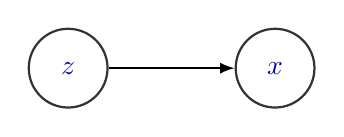
\begin{tikzpicture}
	\tikzstyle{main}=[circle, minimum size = 10mm, thick, draw =black!80, node distance = 16mm]
	\tikzstyle{connect}=[-latex, thick]
	\node[main] (z) [] {$\rvec z$};
	\node[main, fill = black!0] (x) [right=of z] {$\rvec x$};
	\path (z) edge [connect] (x);
	\end{tikzpicture}
	\caption{Prikaz grafičkog modela čija je združena razdioba $p(\vec x, \vec z) = p(\vec z) p(\vec x\mid\vec z)$. }
	\label{fig:pgm}
\end{figure}
%TODO zasjenjen čvor?


\subsection{Varijacijsko zaključivanje}

Za razliku od uzorkovanja kod MCMC-postupaka, osnovna ideja kod varijacijskog zaključivanja je optimizacija. Prvo se odabire familija razdioba $\set{Q}=\cbr{p(\tilde{\rvec z})}_{\tilde{\rvec z}}=\cbr{\mathcal{Q}_{\vec\phi}}_{\vec\phi}$ koje su lakše za računanje. Razdiobe iz $\set{Q}$ su parametrizirane tzv. \emph{varijacijskim parametrima} $\vec\phi$. Cilj je na temelju podataka kao zamjenu za aposteriornu razdiobu $p(\vec z\mid\vec x)$ pronaći razdiobu iz $\set{Q}$ koja ju što bolje aproksimira. To možemo ostvariti minimizacijom Kullback-Leiblerove (KL) divergenciju s obzirom na stvarnu aposteriornu razdiobu po varijacijskim parametrima:
\begin{align}
\mathcal{Q}^* = \argmin_{p(\tilde{\rvec z})\in\set Q} \Dkl{\tilde{\rvec z}}{(\rvec z\mid\vec x)} \text{.}
\end{align}
Ovakva ciljna funkcija obično se ne može lako izračunati jer zahtijeva računanje marginalne izglednosti $p(\vec x)$ iz nazivnika u jednadžbi~\eqref{eq:posterior-inference} marginalizacijom po $\rvec z$, što može biti netraktabilno:
\begin{align}
\Dkl{\tilde{\rvec z}}{(\rvec z\mid\vec x)} 
&= \E_{\tilde{\rvec z}} \ln\frac{p(\tilde{\vec z})}{p(\rvec z\sheq\tilde{\vec z}\mid\vec x)} \nonumber \\
&= \E_{\tilde{\rvec z}} \ln p(\tilde{\vec z}) - \E_{\tilde{\rvec z}}  \ln p(\rvec z\sheq\tilde{\vec z}\mid\vec x) \nonumber\\
&= \E_{\tilde{\rvec z}}  \ln p(\tilde{\vec z}) - \E_{\tilde{\rvec z}}  \ln p(\rvec z\sheq\tilde{\vec z},\vec x) + \ln p(\vec x) \text{.} \label{eq:dkl-split}
\end{align}

Umjesto minimizacije KL-divergencije, možemo maksimizirati funkciju koja se naziva \emph{varijacijska donja granica} (engl. \textit{variational lower bound}) ili \emph{donja granica (logaritma) marginalne izglednosti} (engl. \textit{(log) evidence lower bound}, \textit{ELBO}):
\begin{align}
L_{\rvec x}(\tilde{\rvec z}) 
\coloneqq& \E_{\tilde{\rvec z}} \ln p(\rvec z\sheq\tilde{\vec z},\vec x) - \E_{\tilde{\rvec z}} \ln p(\tilde{\vec z})  \text{.} \label{eq:elbo}
\end{align}
To se i ovako može izraziti:
\begin{align}
L_{\rvec x}(\tilde{\rvec z}) 
= \E_{\tilde{\rvec z}} \ln p(\vec x\mid\rvec z\sheq\tilde{\vec z}) - \Dkl{\tilde{\rvec z}}{\rvec z}  \text{.}
\end{align}
Maksimiziranje takve ciljne funkcije daje razdiobu $p(\tilde{\rvec z})$ koja dobro objašnjava podatke, jer se potiče veće očekivanje logaritma izglednosti, i nije previše daleko od apriorne razdiobe, jer se potiče manja KL-divergencija između varijacijske razdiobe i apriorne razdiobe \citep{Gal:2015:DBAA}. Zamjenom prvih dvaju članova u jednadžbi \eqref{eq:dkl-split},
KL-divergencija se može ovako izraziti:
\begin{align}\label{eq:DklELBO}
\Dkl{\tilde{\rvec z}}{(\rvec z\mid\vec x)} = - L_{\rvec x}(\tilde{\rvec z}) + \ln p(\vec x) \text{.}
\end{align}
Naziv \textit{donja granica marginalne izglednosti} dolazi od toga što su \cite{Jordan:1999:IVMGM} izveli nejednakost $\ln p(\vec x) \geq L_{\rvec x}(\tilde{\rvec z})$ preko Jensenove nejednakosti. Ta nejednakost slijedi i iz prethodne jednadžbe i nenegativnosti KL-divergencije:
\begin{align}
\ln p(\vec x) = L_{\rvec x}(\tilde{\rvec z}) + \Dkl{\tilde{\rvec z}}{(\rvec z\mid\rvec x)} \geq L_{\rvec x}(\tilde{\rvec z}) \text{.}
\end{align}



TODO mean-field, calculus of variations
%https://en.wikipedia.org/wiki/Variational_Bayesian_methods
% https://en.wikipedia.org/wiki/Calculus_of_variations


\subsection{Monte Carlo aproksimacija}

1.3.1 \cite{Neal:1995:BLNN}.



\chapter{Duboko učenje i konvolucijske mreže}


\section{Duboke neuronske mreže}


\section{Konvolucijske mreže}


\section{Optimizacija}

\subsection{Propagacija pogreške unatrag}

\subsection{Isključivanje neurona - dropout}

\subsection{Normalizacija po grupama}



\chapter{Procjenjivanje nesigurnosti}


\section{Aleatorna i epistemička nesigurnost}

Kod bayesovskih modela nesigurnost zaključivanja izražava se razdiobom po vrijednostima varijable čija vrijednost se procjenjuje, a može se izraziti i entropijom ili varijancom kada je prikladno.

Postoje različiti izvori nesigurnosti \citep{Kennedy:2002:BCCM}, ali nesigurnost općenito možemo podijeliti na dvije vrste \citep{Kiureghian:2009:AEDM}: \emph{aleatornu nesigurnost} i \emph{epistemičku nesigurnost}. Riječ \textit{aleatorna} izvedena je od latinske riječi \textit{alea} koja znači \textit{kocka} i asocira na nasumičnost bacanja kocke, a riječ \textit{epistemička} izvedena je od grčke riječi \textit{epist\={e}m\={e}} koja znači \textit{znanje}. Aleatorna nesigurnost je nesigurnost koju model ne može smanjiti neovisno o znanju i količini dostupnih podataka. Ona dolazi od nedeterminizma samog procesa koji generira podatke, nedostupnosti dijela informacija ili ograničenja modela. Epistemička nesigurnost je nesigurnost u parametre modela. Ona dolazi od neznanja i može se smanjiti uz više podataka.

Granica između aleatorne i epistemičke nesigurnosti ovisi o modelu. Nešto što je kod jednostavnijeg modela aleatorna nesigurnost, kod složenijeg modela može biti će epistemičkog karaktera. Ako su neke pojave po prirodi nasumične ili se ne mogu ili ne žele modelu dati informacije koje bi ih mogle objasniti, nesigurnost zaključivanja u vezi tih pojava će, neovisno o ograničenosti modela, biti aleatorna.

TODO: homoskedastička, heteroskedastička nesigurnost

\the\fontdimen5\font\newline % em
\the\fontdimen6\font\newline % ex

\the\textwidth

\begin{figure}
	\centering
	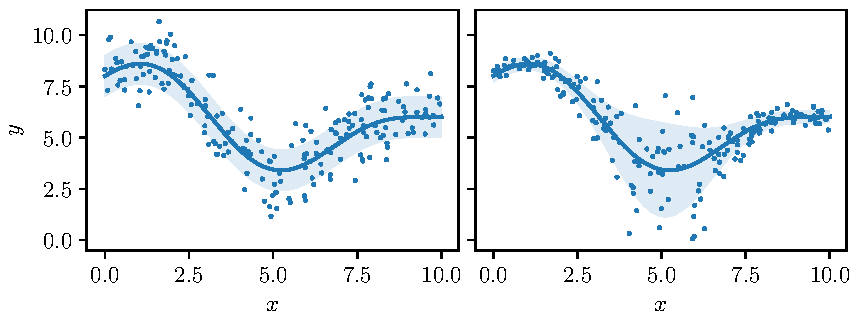
\includegraphics[width=1.0\textwidth]{homoscedastic-heteroscedastic-noises}
	\caption{Homoskedaktički (lijevo) i heteroskedaktički (desno) Gaussov šum.  Crta prikazuje očekivanje $f(x)$, svijetloplava površina standardnu devijaciju šuma $s(x)$, a točke slučajne uzorke. Točke su generirane prema $(\rvar y\mid x) \sim \mathcal{N}(f(x),s(x)^2)$. Na lijevoj slici je $s(x)=1$.}
	\label{fig:homoscedastic-heteroscedastic-noises}
\end{figure}



\chapter{Bayesovske neuronske mreže}



\chapter{Procjenjivanje nesigurnosti kod konvolucijskih mreža}



\chapter{Eksperimentalni rezultati}


\section{Skupovi podataka}



\chapter{Zaključak}

Zaključak.

\bibliography{literatura}
\bibliographystyle{fer}

\begin{sazetak}
Sažetak na hrvatskom jeziku.

\kljucnerijeci{Ključne riječi, odvojene zarezima.}
\end{sazetak}

% TODO: Navedite naslov na engleskom jeziku.
\engtitle{Title}
\begin{abstract}
Abstract.

\keywords{Keywords.}
\end{abstract}

\begin{appendices}
	\chapter{Izvod donje varijacijske granice}
	The contents...
\end{appendices}

\end{document}
